\section{Motivation: Isolating the Visual Grounding Bottleneck}
\label{sec:motivation}

Prior to constructing our agent architecture, we conducted a sequence of controlled ablation experiments designed to isolate the exact computational failure modes where autonomous language model agents squander their action budgets in interactive reasoning tasks.

\paragraph{The Representation Ladder.}
We evaluated a state-of-the-art frontier model (Gemini 1.5 Pro) on the inaugural level of \code{ls20}---a representative ARC-AGI-3 environment featuring a discrete keyboard-navigated maze with directional barriers, an inventory key, a locking mechanism, and a dynamic action gauge. Holding the model, prompt instructions, and underlying environment strictly constant, we systematically modulated only the modality and structure of the input observation (Figure~\ref{fig:gemini}).

\begin{figure}[t]
\centering
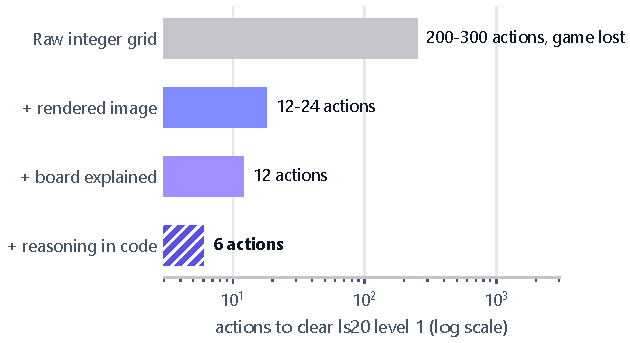
\includegraphics[width=\columnwidth]{figures/gemini_ladder.pdf}
\caption{Controlled ablation of input observation modalities on the first level of \code{ls20}, evaluated using an identical frontier reasoning model. Serializing the environment as raw integer tokens induces catastrophic exploration failure (200--300 actions, exceeding budget). Providing a rendered visual frame reduces required actions by over an order of magnitude (14$\times$ speedup), while augmenting the state with deterministic geometric relations and programmatic execution achieves super-human efficiency (6 actions versus human baseline $\approx$10).}
\label{fig:gemini}
\end{figure}

When provided solely with the raw $64{\times}64$ integer matrix and the valid action enumeration, the model expended between 200 and 300 exploratory actions, repeatedly colliding with invisible topological boundaries and ultimately exhausting the action budget without reaching the goal state. Serializing spatial lattices into discrete token sequences destroys spatial adjacency priors: evaluating topological reachability across 4,096 integer tokens requires quadratic attention across distant positions in the sequence, an operation that autoregressive attention heads fail to execute reliably \citep{rahmanzadehgervi2024blind}. 

Conversely, supplying the identical model with a rendered 2D image of the identical board immediately reduced action expenditure to 12--24 actions---an operational speedup exceeding an order of magnitude achieved purely by aligning the state representation with visual pre-training priors. Augmenting the visual frame with a structural decomposition of board components (delineating static terrain, dynamic gauges, and color parity invariants) further condensed the trajectory to 12 actions. Finally, prompting the model to synthesize programmatic search scripts within an execution sandbox yielded optimal completion in exactly 6 actions. The primary performance leap stems from perceptual grounding rather than scale of reasoning.

\paragraph{The Oracle Briefing: Decoupling Perception from Planning.}
To determine whether agent failures originate from deficiencies in high-level policy planning or low-level perceptual parsing, we performed an oracle comprehension experiment. The model was tasked with solving an advanced level of \code{ls20} under two conditions: (i) providing visual screenshots alone, and (ii) augmenting visual screenshots with an ``oracle briefing''---a concise, structured natural language annotation specifying inferred action semantics, goal criteria, mechanical dependencies, and identified on-screen entities.

Without the briefing, the agent squandered its entire action allocation exploring inert visual artifacts and failed to resolve the level. In the presence of the structural briefing, the model formulated an optimal plan and cleared the level in 6 actions, substantially outperforming the author's initial blind playthrough ($\approx$10 actions). This empirical divergence establishes a vital architectural insight: modern reasoning backbones possess highly capable sequential planning and programmatic search capabilities, but their execution remains bottlenecked by inaccurate visual state induction. If an agent can be provided with high-fidelity semantic and geometric grounding, its downstream planning executes with near-optimal efficiency.

\paragraph{The Failure of Sparse Coordinate Deltas.}
In resource-constrained settings, a common optimization is transmitting only sparse coordinate deltas (i.e., the set of grid cells modified between step $t-1$ and $t$) to minimize prompt token consumption. While computationally economical, our empirical tracking revealed that coordinate deltas induce severe perceptual myopia. In ARC-AGI-3 environments, local agent actions routinely trigger non-local, global state transitions: for example, stepping onto a localized trigger tile in \code{ls20} instantaneously alters an icon situated in a distant status panel. When an agent receives only localized coordinate updates, it systematically overlooks global mechanical coupling, hallucinating that its action produced no operational side-effects. Maintaining holistic whole-frame visual representations is therefore mandatory to preserve causal tracking across the entire visual field.

\paragraph{Core Design Principles of the Perception Engine.}
Because oracle briefings cannot exist for undisclosed, held-out environments during official evaluation, an autonomous agent must construct its own structural abstractions dynamically. ARC-AGI-3 environments are strictly grounded in human core knowledge \citep{spelke2007core}, which is predominantly geometric and topological: connectivity, spatial enclosure, lattice-constrained reachability, structural symmetry, and affine transformations. 

These properties admit exact, deterministic algorithmic verification. In contrast, operational semantics (e.g., identifying which dynamic component represents the agent embodiment, or what constitutes the terminal win condition) are fundamentally latent under partial observability and can only be induced through empirical interaction. 

These findings dictate the central architectural axiom governing \textsc{Sarbloh}:
\begin{quote}
\itshape
Compute mathematically certain geometric invariants deterministically via zero-parameter host code; formulate ambiguous operational roles as explicit probabilistic hypotheses; and equip every hypothesis with a minimal-cost, single-action falsification test.
\end{quote}
By enforcing this strict dichotomy, the agent eliminates visual hallucination over spatial facts, while ensuring that any incorrect operational hypothesis is refuted through a single probing action, entirely averting catastrophic quadratic exploration penalties.